% ------------------------------------------------------ %
%  BIOE60009 Physiological Fluid Mechanics 
%  Formula Booklet                                       
% ------------------------------------------------------ %
% This work is licensed under a Creative Commons Attribution 4.0 International License 
% ------------------------------------------------------ %
% AUTHORS
%           Binghuan Li  <binghuan.li19@imperial.ac.uk>, 
%           Peter Xie    <peter.xie19@imperial.ac.uk>
% ------------------------------------------------------ %
% FIRST RELEASE        May 17, 2022                 
% ------------------------------------------------------ %
% ------------------------------------------------------ %

\documentclass{article}
\usepackage[margin=2cm]{geometry}
\usepackage{amsmath}
\usepackage{amsfonts}
\usepackage{mathrsfs} 
\usepackage{mathtools} 
\DeclareMathOperator{\sech}{sech}
\DeclareMathOperator{\arctanh}{artanh}
\DeclareMathOperator{\cosec}{cosec}
\DeclareMathOperator{\arcsinh}{arsinh}
\usepackage{amssymb}
\usepackage{fancyhdr}
\usepackage{siunitx}
\usepackage{enumitem}
\usepackage{hyperref}
\usepackage{graphicx}
\usepackage{float}
\usepackage{framed}
\hypersetup{pdfauthor={Li, Binghuan}}
\pagestyle{fancy}
\fancyhf{}
\lhead{\textsc{Physiological Fluid Mechanics Cheat Sheet}}
\rhead{page \thepage}

\usepackage{tcolorbox}
\usepackage[utf8]{inputenc}
\usepackage[sfdefault]{arimo}
\usepackage[T1]{fontenc}

\usepackage{tikz}
\usepackage{circuitikz}

\usepackage{multicol}
\setlength{\columnseprule}{1pt}

\usepackage{lscape}

\begin{document}

\section{Tensors, Notations}
\begin{multicols}{2}
\begin{enumerate}

    \item Kronecker delta: 
    \begin{align*}
    \delta_{ij} = 
        \begin{cases}
            1 & \text{if} \ i=j \\
            0 & \text{if} \ i\neq j \\
        \end{cases}
    \end{align*}
    Properties:
    \[\delta_{ij}x_{j} = x_{i} \quad \delta_{ij}=\delta_{ji}\]
    
    \item Alternating tensor:
    \begin{align*}
    \epsilon_{ijk} = 
        \begin{cases}
            1 & \{ijk\} \ =\ \{1,2,3\}, \{2,3,1\}, \{3,1,2\} \\
            -1 & \{ijk\} \ =\ \{3,2,1\}, \{2,1,3\}, \{1,3,2\} \\
            0 & \text{otherwise}
        \end{cases}
    \end{align*}
    Properties:
    \[\epsilon_{ijk}\epsilon_{klm} = \delta_{il}\delta_{jm}-\delta_{im}\delta_{kl}\]
    \[\epsilon_{ijk} = -\epsilon_{ikj}\]
    
    \item Dot product: \[\mathbf{a} \cdot \mathbf{b} = a_{i}b_{i}\]
    
    \item Cross product: \[\mathbf{a} \times \mathbf{b} = \epsilon_{ijk}a_{j}b_{k}\]
    
    \item Gradient operator: \[\nabla f = \frac{\partial f_{i}}{\partial x_{j}} \quad \quad (\nabla T)_{ijk} = \frac{\partial T_{jk}}{\partial x_{i}}\]
    
    \item Divergence operator: \[\nabla \cdot f = \frac{\partial f_{i}}{\partial X_{i}} \quad \quad (\nabla \cdot T)_{j} = \frac{\partial T_{ij}}{\partial x_{i}}\]
    
    \item Curl operator: \[\nabla \times f = \epsilon_{ijk} \frac{\partial}{\partial x_{j}}f_{k} \]
    
    \item Properties:
    \[f_{i}\frac{\partial \phi}{\partial x_{i}} = f\cdot \nabla \phi\]
    \[f_{k}\frac{\partial f_{i}}{\partial f_{k}} = (f\cdot \nabla)f\]
    \[\nabla\cdot(\nabla \times f) = 0\]
    \[\nabla \times \nabla = 0\]

\end{enumerate}
\end{multicols}


\section{Constitutive Relations for Newtonian Fluids}
\begin{enumerate}
    \item \textbf{Stress Tensor:}
      \[\sigma_{ij} = \underbrace{-p\delta_{ij}}_{\text{pressure}} + \underbrace{d_{ij}}_{\text{Deviatoric stress}} \]
      where $i$ = surface orientation, $j$ = direction of force.
 
    \item \textbf{Fluid Strain Rate Tensor:}
      \begin{equation*}
          \mathbf{e} = \frac{1}{2}(\frac{\partial u_{i}}{\partial x_{j}} + \frac{\partial u_{j}}{\partial x_{i}})=\frac{1}{2}(\nabla \mathbf{u}+(\nabla \mathbf{u})^{T})
          \quad \quad
          \mathbf{e} = 
          \begin{pmatrix}
          \frac{\partial u}{\partial x} & \frac{1}{2}(\frac{\partial u}{\partial y}+\frac{\partial v}{\partial x}) & \frac{1}{2}(\frac{\partial u}{\partial z}+\frac{\partial w}{\partial x})\\[0.5em]
          
          \frac{1}{2}(\frac{\partial u}{\partial y}+\frac{\partial v}{\partial x}) & \frac{\partial v}{\partial y}  & \frac{1}{2}(\frac{\partial v}{\partial z}+\frac{\partial w}{\partial y})\\[0.5em]
          
          \frac{1}{2}(\frac{\partial u}{\partial z}+\frac{\partial w}{\partial x}) & \frac{1}{2}(\frac{\partial v}{\partial z}+\frac{\partial w}{\partial y})  & \frac{\partial w}{\partial z}\\
          \end{pmatrix}
      \end{equation*}

      \begin{equation*}
          \mathbf{e} = 
          \begin{pmatrix}
          \frac{\partial u_{r}}{\partial r} & \frac{1}{2}(r\frac{\partial (u_{\theta}/r)}{\partial r}+\frac{1}{r}\frac{\partial u_{r}}{\partial \theta}) & \frac{1}{2}(\frac{\partial u_{z}}{\partial r}+\frac{\partial u_{r}}{\partial z})\\[0.5em]
          
          \frac{1}{2}(r\frac{\partial (u_{\theta}/r)}{\partial r}+\frac{1}{r}\frac{\partial u_{r}}{\partial \theta}) & \frac{1}{r}\frac{\partial u_{\theta}}{\partial \theta}+\frac{u_{r}}{r} & \frac{1}{2}(\frac{\partial u_{\theta}}{\partial r}+\frac{1}{r}\frac{\partial u_{z}}{\partial \theta})\\[0.5em]
          
          \frac{1}{2}(\frac{\partial u_{z}}{\partial r}+\frac{\partial u_{r}}{\partial z}) & \frac{1}{2}(\frac{\partial u_{\theta}}{\partial r}+\frac{1}{r}\frac{\partial u_{z}}{\partial \theta})  & \frac{\partial u_{z}}{\partial z}\\
          \end{pmatrix}
      \end{equation*}

    \item \textbf{Fluid Constitutive Relationship:} relation between force and deformation
      \[ \sigma_{ij} = -p\delta_{ij} + \lambda \delta_{ij} \underbrace{\frac{\partial u_{k}}{\partial x_{k}}}_{\nabla \cdot \mathbf{u}} + \mu \underbrace{(\frac{\partial u_{i}}{\partial x_{j}} + \frac{\partial u_{j}}{\partial x_{i}})}_{\text{strain rate}, 2\mathbf{e}} = -p\mathbf{I} + \lambda (\nabla \cdot \mathbf{u})\mathbf{I} + 2\mu \mathbf{e}\]
      
    \item \textbf{Cauchy's Equation:} apply Newton's 2\textsuperscript{nd} Law to constitutive relationship
      \[  \rho (\frac{\partial u}{\partial t} + u \cdot \nabla u) = \nabla \cdot \sigma + \rho f \]
      Expanding Cauchy's equation produces the Navier-Stokes momentum equation
    %   \item Non-Newtonian Fluids\\
    %   Blood viscosity ($\mu$) is dependent on strain rate, stress history (viscoelasticity), Hematocrit, disease, and heat.
\end{enumerate}


\section{Navier-Stokes Equations}

    \subsection{Momentum Equation}
        \[\rho \bigg( \frac{\partial u_{i}}{\partial t} + u_{j}\frac{\partial u_{i}}{\partial x_{j}} \bigg) = -\frac{\partial p}{\partial x_{i}} + \mu \frac{\partial u_{i}}{\partial x_{j}\partial x_{j}} + \rho f_{i}\]

        \begin{multicols}{2}
        \begin{itemize}
            \item[-] $\frac{\partial u_{i}}{\partial t}$: Unsteady term. Acceleration (with respect to space) at a particular location.
    
            \item[-] $u_{j}\frac{\partial u_{i}}{\partial x_{j}}$: Convective acceleration term. Acceleration with respect to space.
    
            \item[-] $\frac{\partial p}{\partial x_{i}}$: Pressure gradient. Main driver of flow.
        
            \item[-] $\mu \frac{\partial u_{i}}{\partial x_{j}\partial x_{j}}$: Viscous term. Viscosity imply resistance to flow.
    
            \item[-] $\rho f_{i}$: Body force term. Gravity, electromagnetism etc.
        \end{itemize}
        \end{multicols}
        Due to the convective acceleration term, Navier-Stokes equation is non-linear, therefore, they cannot be decomposed using basis functions (\textit{e.g.} Fourier series).
        
    \subsection{Energy Equation}
        \[\rho c_{v} \bigg(\frac{\partial T}{\partial t} + \mathbf{u}\cdot \nabla T \bigg) = k\nabla^{2}T + \Phi + \dot{S} \]
        
        \begin{multicols}{2}
        \begin{itemize}
            \item[-] $\frac{\partial T}{\partial t}$: rate of change of heat at a particular location
    
            \item[-] $u\cdot \nabla T$: heat convection. How much heat is being brought about by moving fluid velocities?
    
            \item[-] $k\nabla^{2}T$: Heat conduction. 
        
            \item[-] $\Phi$: Work done by fluid shear and pressure.
    
            \item[-] $\dot{S}$: Energy production.
        \end{itemize}
        \end{multicols}
        
        
    \subsection{Cartesian Coordinates} 
        \begin{itemize}
            \item Continuity Equation:
            \[\frac{\partial u}{\partial x} + \frac{\partial v}{\partial y} + \frac{\partial w}{\partial z}=0\]
            
            \item Momentum Equations:
            \[\rho \bigg(\frac{\partial \mathbf{u}}{\partial t} + (\mathbf{u}\cdot \nabla)\mathbf{u} \bigg) = -\nabla p + \mu \nabla^{2}\mathbf{u} + \rho \mathbf{f}\]
            
            \[x: \ \rho \bigg(\frac{\partial u}{\partial t} + u \frac{\partial u}{\partial x} + v\frac{\partial u}{\partial y} + w\frac{\partial u}{\partial z} \bigg) = -\frac{\partial p}{\partial x} + \mu \bigg(\frac{\partial^{2} u}{\partial x^{2}} + \frac{\partial^{2} u}{\partial y^{2}} + \frac{\partial^{2} u}{\partial z^{2}}\bigg) + \rho f_{x}\]
            
            \[y: \ \rho \bigg(\frac{\partial v}{\partial t} + u \frac{\partial v}{\partial x} + v\frac{\partial v}{\partial y} + w\frac{\partial v}{\partial z} \bigg) = -\frac{\partial p}{\partial y} + \mu \bigg(\frac{\partial^{2} v}{\partial x^{2}} + \frac{\partial^{2} v}{\partial y^{2}} + \frac{\partial^{2} v}{\partial z^{2}}\bigg) + \rho f_{y}\]
            
            \[z: \ \rho \bigg(\frac{\partial w}{\partial t} + u \frac{\partial w}{\partial x} + v\frac{\partial w}{\partial y} + w\frac{\partial w}{\partial z} \bigg) = -\frac{\partial p}{\partial z} + \mu \bigg(\frac{\partial^{2} w}{\partial x^{2}} + \frac{\partial^{2} w}{\partial y^{2}} + \frac{\partial^{2} w}{\partial z^{2}}\bigg) + \rho f_{z}\]
            
            \item Energy Equation:
            \[\rho c_{v} \bigg(\frac{\partial T}{\partial t} + \mathbf{u}\cdot \nabla T \bigg) = k\nabla^{2}T + \Phi + \dot{S} \]
        \end{itemize}
    
    \subsection{Cylindrical Coordinates} 
        \begin{itemize}
            \item Continuity Equation:
            \[\frac{1}{r}\frac{\partial ru_{r}}{\partial r} + \frac{1}{r}\frac{\partial u_{\theta}}{\partial \theta} + \frac{\partial u_{z}}{\partial z}=0\]
            
            \item Momentum Equations:
            
            \[r: \ \rho \bigg(\frac{\partial u_{r}}{\partial t} + u_{r} \frac{\partial u_{r}}{\partial r} + \frac{u_{\theta}}{r}\frac{\partial u_{r}}{\partial \theta} + u_{z}\frac{\partial u_{r}}{\partial z} - \frac{u_{\theta}^{2}}{r} \bigg) = -\frac{\partial p}{\partial r} + \mu \bigg[ \frac{1}{r}\frac{\partial}{\partial r} \bigg(r \frac{\partial u_{r}}{\partial r}\bigg) + \frac{1}{r^{2}} \frac{\partial^{2} u_{r}}{\partial \theta^{2}} + \frac{\partial^{2} u_{r}}{\partial z^{2}} - \frac{u_{r}}{r^{2}} - \frac{2}{r^{2}}\frac{\partial u_{\theta}}{\partial \theta}\bigg] + \rho f_{r}\]
            
            \[\theta: \ \rho \bigg(\frac{\partial u_{\theta}}{\partial t} + u_{r} \frac{\partial u_{\theta}}{\partial r} + \frac{u_{\theta}}{r} \frac{\partial u_{\theta}}{\partial \theta} + u_{z}\frac{\partial u_{\theta}}{\partial z} + \frac{u_{r}u_{\theta}}{r} \bigg) = -\frac{1}{r} \frac{\partial p}{\partial \theta} + \mu \bigg[ \frac{1}{r}\frac{\partial}{\partial r} \bigg(r \frac{\partial u_{\theta}}{\partial r}\bigg) + \frac{1}{r^{2}} \frac{\partial^{2} u_{\theta}}{\partial \theta^{2}} + \frac{\partial^{2} u_{\theta}}{\partial z^{2}} - \frac{u_{\theta}}{r^{2}} + \frac{2}{r^{2}}\frac{\partial u_{r}}{\partial \theta}\bigg] + \rho f_{\theta}\]
            
            \[z: \ \rho \bigg(\frac{\partial u_{z}}{\partial t} + u_{r} \frac{\partial u_{z}}{\partial r} + \frac{u_{\theta}}{r}\frac{\partial u_{z}}{\partial \theta} + u_{z}\frac{\partial u_{z}}{\partial z} \bigg) = -\frac{\partial p}{\partial z} + \mu \bigg[ \frac{1}{r}\frac{\partial}{\partial r} \bigg(r \frac{\partial u_{z}}{\partial r}\bigg) + \frac{1}{r^{2}} \frac{\partial^{2} u_{z}}{\partial \theta^{2}} + \frac{\partial^{2} u_{z}}{\partial z^{2}} \bigg] + \rho f_{z}\]
        \end{itemize}
    
    \subsection{Spherical Coordinates}
        \begin{itemize}
            \item Continuity Equation:
            \[\frac{1}{r^{2}}\frac{\partial r^{2}u_{r}}{\partial r} + \frac{1}{r \sin \theta}\frac{\partial u_{\theta}\sin \theta}{\partial \theta} + \frac{1}{r \sin \theta}\frac{\partial u_{\phi}}{\partial \phi}=0\]
            
            \item Momentum Equations:
            
            \begin{equation*}
            \begin{split}
            r: \ & \rho \bigg(\frac{\partial u_{r}}{\partial t} + u_{r} \frac{\partial u_{r}}{\partial r} + \frac{u_{\theta}}{r}\frac{\partial u_{r}}{\partial \theta} + \frac{u_{\phi}}{r \sin \theta} \frac{\partial u_{r}}{\partial \phi} - \frac{u_{\theta}^{2}+u_{\phi}^{2}}{r} \bigg)  \\ 
            & = -\frac{\partial p}{\partial r} + \mu \bigg( \nabla^{2}u_{r} - \frac{2u_{r}}{r^{2}} - \frac{2}{r^{2}\sin \theta}\frac{\partial}{\partial \theta}(u_{\theta}\sin\theta) + \frac{2}{r^{2}\sin\theta}\frac{\partial u_{\phi}}{\partial \phi} \bigg) + \rho f_{r}
            \end{split}  
            \end{equation*}
            
            \begin{equation*}
            \begin{split}
            \theta: \ & \rho \bigg(\frac{\partial u_{\theta}}{\partial t} + u_{r} \frac{\partial u_{\theta}}{\partial r} + \frac{u_{\theta}}{r} \frac{\partial u_{\theta}}{\partial \theta} + \frac{u_{\phi}}{r\sin \theta} \frac{\partial u_{\theta}}{\partial \phi} + \frac{u_{r}u_{\theta}-u_{\phi}^{2}\cot\theta}{r} \bigg) \\
            & = -\frac{1}{r}\frac{\partial p}{\partial \theta} + \mu \bigg( \nabla^{2}u_{\theta} - \frac{u_{\theta}}{r^{2}\sin^{2}\theta} + \frac{2}{r^{2}}\frac{\partial u_{r}}{\partial \theta} - \frac{2\cos \theta}{r^{2}\sin^{2}\theta}\frac{\partial u_{\phi}}{\partial \phi} \bigg) + \rho f_{\theta}
            \end{split}  
            \end{equation*}
            
            \begin{equation*}
            \begin{split}
            \phi: \ & \rho \bigg(\frac{\partial u_{\phi}}{\partial t} + u_{r} \frac{\partial u_{\phi}}{\partial r} + \frac{u_{\theta}}{r} \frac{\partial u_{\phi}}{\partial \theta} + \frac{u_{\phi}}{r\sin \theta} \frac{\partial u_{\phi}}{\partial \phi} + \frac{u_{r}u_{\phi}+u_{\phi}u_{\theta}\cot\theta}{r} \bigg) \\
            & = -\frac{1}{r\sin\theta}\frac{\partial p}{\partial \phi} + \mu \bigg( \nabla^{2}u_{\phi} - \frac{u_{\phi}}{r^{2}\sin^{2}\theta} + \frac{2}{r^{2}\sin \theta}\frac{\partial u_{r}}{\partial \phi} - \frac{2\cos \theta}{r^{2}\sin^{2}\theta}\frac{\partial u_{\theta}}{\partial \phi} \bigg) + \rho f_{\phi}
            \end{split}  
            \end{equation*}
        \end{itemize}


\section{Assumptions with Navier-Stokes Equations}
\begin{multicols}{2}
\begin{itemize}
    \item Steady flow: $\displaystyle \frac{\partial}{\partial t} = 0$
    \item Fully developed flow: $\displaystyle \frac{\partial}{\partial z} = 0$
    \item Axisymmetric flow: $\displaystyle \frac{\partial}{\partial \theta} = 0$
    \item Spherical symmetric flow: $\displaystyle \frac{\partial}{\partial \theta} = 0, \frac{\partial}{\partial \phi} = 0$
    \item No Swirl: $u_{\theta} = 0$
    \item Two-dimensional flow: $\displaystyle u_{z}=0$ and $\displaystyle \frac{\partial}{\partial z} = 0$
\end{itemize}
\end{multicols}

\section{Womersley Solution}
\textbf{Assumptions: }
axisymetric: $\displaystyle \frac{\partial}{\partial \theta}=0$; 
fully developed: $\displaystyle \frac{\partial u_{r}}{\partial z}=0$; 
lower limit, converges to steady flow (Hagen-Poiseuille flow Eqn, parabolic flow): $\displaystyle \frac{\partial}{\partial t}=0$; $u_{r}=0$; Higher limit converges to stokes flow derivation.  
no swirl: $u_{\phi}=0$.
\begin{itemize}
    \item Final solution is \[U(r) = \frac{iG_{0}}{2\omega \rho}\bigg[ 1- \frac{J_{0}(i^{3/2}\alpha 
    \frac{r}{a})}{J_{0}(i^{3/2}\alpha)} \bigg]\]
    
    \[u_{z}(r,t) = \frac{i}{\omega \rho} \frac{\partial p}{\partial z} \bigg[ 1- \frac{J_{0}(i^{3/2}\alpha 
    \frac{r}{a})}{J_{0}(i^{3/2}\alpha)} \bigg] e^{i\omega t} = \frac{iG_{0}}{2\omega \rho}\bigg[ 1- \frac{J_{0}(i^{3/2}\alpha 
    \frac{r}{a})}{J_{0}(i^{3/2}\alpha)} \bigg] \]
    
    \noindent \textbf{Wormersley number:} $\displaystyle \alpha = a \sqrt{\frac{\omega}{\nu}}$,  non-dimensional, ratio between unsteady inertia force to viscous force.
    
    \item Wall shear stress: \[\tau_{rz} = \mu \frac{\partial u_{z}}{\partial r} = Re\bigg\{ -\frac{a}{i^{3/2}\alpha} \bigg( \frac{J_{1}(i^{3/2}\alpha)}{J_{0}(i^{3/2}\alpha)} \bigg) \frac{\partial p}{\partial z} \bigg\}\]
    
    \item Volume flow rate: \[Q(t) = \int_{0}^{a} 2\pi r u_{z} \mathrm{d}r = Re\bigg\{ -\frac{\pi a^{4}}{i \mu \alpha^{2}} \bigg( 1 - \frac{2J_{1}(i^{3/2}\alpha)}{\alpha i^{3/2} J_{0}(i^{3/2}\alpha)} \bigg) \frac{\partial p}{\partial z} \bigg\}\]
    
    Useful Bessel function property: $\displaystyle \frac{\partial J_{0}(s)}{\partial s} = -J_{1}(s)$
\end{itemize}

% \begin{figure}[H]
%     \centering
%     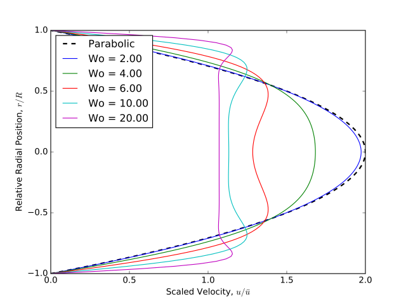
\includegraphics[width=.5\textwidth]{img/womersley.png}
%     \caption{Womersley Solution}
%     \label{fig:my_label}
% \end{figure}

\section{Laminar and Turbulent Pipe Flow}
\begin{itemize}
\item \textbf{Reynolds Number:}
    \[ Re = \frac{\rho VD}{\mu} = \frac{VD}{\nu}\]
    
\item \textbf{Entrance Length:}
    A. Laminar Flow: \[ \frac{L_{e}}{D} = 0.006 Re \]
    B. Turbulent Flow: \[ \frac{L_{e}}{D} = 1.6 Re^{\frac{1}{4}} \]
    
\item \textbf{Head Loss:}
Head loss is the energy loss ($h_{f}$) due to fluid friction.\\
Darcy Friction factor:
\[ h_{f} = f\frac{L}{D}\frac{V^{2}}{2g}\]
where Darcy Friction factor = f. f = function(Re, wall roughness, duct shape)\\
$ f = \frac{64}{Re}$ for laminar flow
\end{itemize}

\begin{landscape}
\begin{figure}
    \centering
    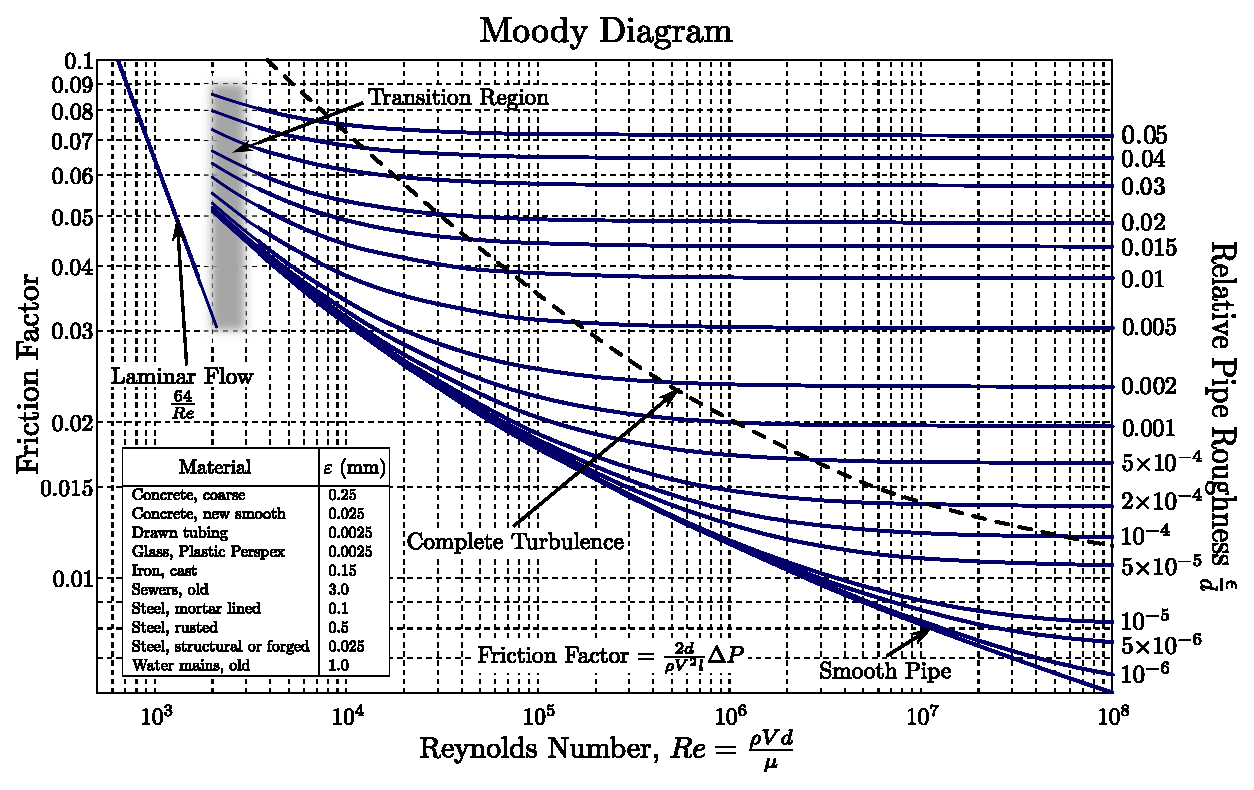
\includegraphics{img/Moody_EN.eps}
    \caption{Moody's chart}
    \label{fig:moody}
\end{figure}
\end{landscape}






\section{Lumped Parameter Methods}
\begin{table}[H]
    \centering
    \begin{tabular}{|c|c|c|} \hline 
        Resistance & Compliance & Inertance  \\ [.2em]\hline 
        $Q = \Delta p / R$ & $Q = C \frac{\partial p}{\partial t}$ & $p = L \frac{\partial Q}{\partial t}$ \\ [.2em] \hline
    \end{tabular}
\end{table}

\subsection{Windkessel Modelling}
\subsubsection{2-element Windkessel Model}
\begin{minipage}{0.5\textwidth}
\begin{center}
    \begin{circuitikz}
    \draw (0,0) to[vsourcesin, sV=$p(t)$] (0,1) -- (0, 2) to [short, i_=$Q_{\rm in}$] (2,2)-- (2,1.5) -- (1.5, 1.5);
    \draw (2, 1.5) -- (2.5, 1.5);
    \draw (1.5, 1.5) to [resistor, R=$R$, o-o] (1.5, -1) -- (2, -1);
    \draw (2.5, 1.5) to [capacitor, C=$C$, o-o] (2.5, -1) -- (2, -1) -- (2, -1.5) -- (0, -1.5) -- (0,0);
    \end{circuitikz}
\end{center}
\end{minipage}
\hfill
\begin{minipage}{0.5\textwidth}
\textbf{Governing Equation:}
\[\frac{dp}{dt} + \frac{p}{RC_{0}} = \frac{Q_{in}}{C_{0}}\]
where $C=dV/dt$ is compliance, $R$ is peripheral resistance.
\end{minipage}

\subsubsection{3-element Windkessel Model}
\begin{minipage}{0.5\textwidth}
\begin{center}
    \begin{circuitikz}
    \draw (-1,0) to[vsourcesin, sV=$p(t)$] (-1,1) -- (-1, 2)node[label={$p$}]{} to [resistor, R=$Z_{c}$, o-o, european](1,2)node[label={$p_{d}$}]{} -- (2,2)-- (2,1.5) -- (1, 1.5);
    \draw (2, 1.5) -- (3, 1.5);
    \draw (1, 1.5) to [resistor, R=$R$, o-o] (1, -1) -- (2, -1);
    \draw (3, 1.5) to [capacitor, C=$C_{0}$, o-o] (3, -1) -- (2, -1) -- (2, -1.5) -- (-1, -1.5) -- (-1,0);
    \end{circuitikz}
\end{center}
\end{minipage}
\hfill
\begin{minipage}{0.5\textwidth}
\textbf{Governing Equation:}
\[\frac{\partial p}{\partial t}+\frac{p}{RC} = \frac{Q}{C}(1+\frac{Z_{c}}{R})+Z_{c}\frac{\partial Q}{\partial t}\]
where $Z_{c}$ is characteristic impedance, $p-p_{d} = Z_{c}Q$ 
\end{minipage}


\subsubsection{4-element Windkessel Model}
\begin{minipage}{0.5\textwidth}
\begin{center}
    \begin{circuitikz}
    \draw (0,0) to[vsourcesin, sV=$p(t)$] (0,1) -- (0, 2)node[label={$p$}]{} -- (1,2) -- (1, 2.5)  to[resistor, R=$Z_{c}$, o-o, european](3, 2.5) -- (3, 2);
    \draw (1,2) -- (1, 1.5) 
    to[inductor, L=$L$, o-o](3, 1.5) -- (3,2) 
    -- (4, 2)node[label={$p_{d}$}]{} -- (4, 1.5) ;
    \draw (4, 1.5) -- (3.5, 1.5) to [resistor, R=$R$, o-o] (3.5, -1) -- (4, -1);
    \draw (4, 1.5) -- (4.5, 1.5) to [capacitor, C=$C_{0}$, o-o] (4.5, -1) -- (4, -1) -- (4, -1.5) -- (0, -1.5) -- (0,0);
    \end{circuitikz}
\end{center}
\end{minipage}
\hfill
\begin{minipage}{0.5\textwidth}
\textbf{Governing Equation:}
\[\frac{\partial p}{\partial t}+\frac{p}{RC} = \frac{Q}{C}(1+\frac{Z_{total}}{R})+Z_{total}\frac{\partial Q}{\partial t}\]
where $\displaystyle Z_{total} = \frac{j\omega L Z_{c}}{j\omega L + Z_{c}}$ is the total impedance of the parallel network - the characteristic impedance, $Z_{c}$ and the inductor, $L$. 
\end{minipage}


%%
\section{Non-Dimensional Navier Stokes Equation}
\begin{itemize}
    \item Non-Dimensional Navier Stokes Equation:\\
     \[ Re\bigg(\frac{\partial \mathbf{u^{*}}}{\partial t^{*}} + (\mathbf{u^{*}}\cdot \nabla^{*})\mathbf{u^{*}} \bigg) = -\frac{P_{0}}{\frac{\mu U}{L}}\nabla^{*} p^{*} + \nabla^{*2}\mathbf{u^{*}}\]
where $\displaystyle P_{0} = \frac{\mu U}{L}max(1,Re)$
     \[ \nabla^{*} \cdot u^{*} = 0\]
     
     \item Small Reynolds number flow (Stokes Equation):
     \[\mu \nabla^{2}\mathbf{u} = \nabla p
     \quad \quad
     \nabla \cdot u = 0\]

     \item High Reynolds number flow:
     \[ \bigg(\frac{\partial \mathbf{u^{*}}}{\partial t^{*}} + (\mathbf{u^{*}}\cdot \nabla^{*})\mathbf{u^{*}} \bigg) = -\nabla^{*} p^{*}
     \quad \quad
     \nabla^{*} \cdot u^{*} = 0\]
    
    \item Lubrication Equations:
    \[\frac{\partial u}{\partial x} + \frac{\partial v}{\partial y} = 0 
    \quad \quad 
    0 = -\frac{\partial p}{\partial x} + \mu \frac{\partial^{2} u}{\partial y^{2}}\]
\end{itemize}


\section{Porous Media Flow}
\begin{itemize}
 \item Darcy Equation:\\
 \begin{minipage}{0.5\textwidth}
 \[\mathbf{u} = -\frac{k}{\mu} \nabla p\]
 \end{minipage}
 \begin{minipage}{0.4\textwidth}
    \begin{itemize}
    \begin{framed}
        \item $\mathbf{u}$ - volume flux per unit area
        \item $\mu$ - Shear viscosity
        \item $k$ - Permeability
    \end{framed}
    \end{itemize}
 \end{minipage}
\end{itemize}


\section{Mass Transport}
\begin{enumerate}
    \item Convection Diffusion Equation\\
    \begin{minipage}{0.5\textwidth}
    \[ \underbrace{\frac{\partial c}{\partial t}}_{\text{rate of change}} + \underbrace{(\mathbf{u} \cdot \nabla) c}_{\text{convection}} =  \underbrace{D \nabla^{2} c}_{\text{diffusion}} - \underbrace{f(c)}_{\text{consumption}} \] 
    \end{minipage}
    \begin{minipage}{0.4\textwidth}
    \begin{itemize}
    \begin{framed}
        \item $c$ - concentration of solute
        \item $\mathbf{u}$ - velocity vector
        \item $D$ - diffusion coefficient
        \item $f$ - consumption of solute
    \end{framed}
    \end{itemize}
    \end{minipage}
    
    \item Reynolds Transport Theorem
    \[ \frac{dB_{sys}}{dt}=\frac{\partial}{\partial t}\int\limits_{CV}\rho \beta dV+\oint\limits_{CS}\rho\beta(\mathbf{v}\cdot\mathbf{n})\mathrm{d}A \]



\end{enumerate}
\vfill
\fbox{Update: \today}
\end{document}